\documentclass[twoside,a4paper,12pt]{mwbk}

\usepackage{polski}
\usepackage[utf8]{inputenc}
%\usepackage{times}
\usepackage{amsmath,amssymb,amsthm}
\usepackage{xcolor}
\usepackage[final]{pdfpages}
\usepackage{graphicx}
%\usepackage[nottoc]{tocbibind}
\usepackage{caption}
\usepackage{subcaption}
\captionsetup{compatibility=false}
\usepackage{dsfont}
\usepackage{float}
%\usepackage{geometry}
%\newgeometry{tmargin=2.5cm, bmargin=2.5cm, lmargin=2.5cm, rmargin=2.5cm}

%\numberwithin{equation}{section}
%\numberwithin{figure}{section}
\renewcommand{\thefigure}{\thechapter.\arabic{figure}}

%\newcommand*{\doi}[1]{\href{http://dx.doi.org/#1}{doi: #1}}
%\newcommand*{\MR}[1]{\href{http://www.ams.org/mathscinet-getitem?mr=#1&return=pdf}{MR #1}}
%\newcommand*{\ZBL}[1]{\href{http://www.zentralblatt-math.org/zmath/en/advanced/?q=an:#1&format=complete}{Zbl #1}}


\newcommand{\1}[1]{\mathds{1}\left(#1\right)}

\newenvironment{diagrams}[2]{\begin{figure}[H]
	%\centering
	\begin{subfigure}{.5\textwidth}
		\centering
		\includegraphics[width=.9\textwidth]{wykresy/#1.png}
		\caption{}
		\label{#1}
	\end{subfigure}
	\begin{subfigure}{.5\textwidth}
		\centering
		\includegraphics[width=.9\textwidth]{wykresy/#2.png}
		\caption{}
		\label{#2}
	\end{subfigure}
	}
	{
	\end{figure}
	}

\newenvironment{subdiagrams}[2]{
		\begin{subfigure}{.5\textwidth}
			\centering
			\includegraphics[width=.9\textwidth]{wykresy/#1.png}
			\caption{}
			\label{#1}
		\end{subfigure}
		\begin{subfigure}{.5\textwidth}
			\centering
			\includegraphics[width=.9\textwidth]{wykresy/#2.png}
			\caption{}
			\label{#2}
		\end{subfigure}
	} {}


\begin{document}
	
\begin{titlepage}
	
\includepdf{StronaTytulowa.pdf}
	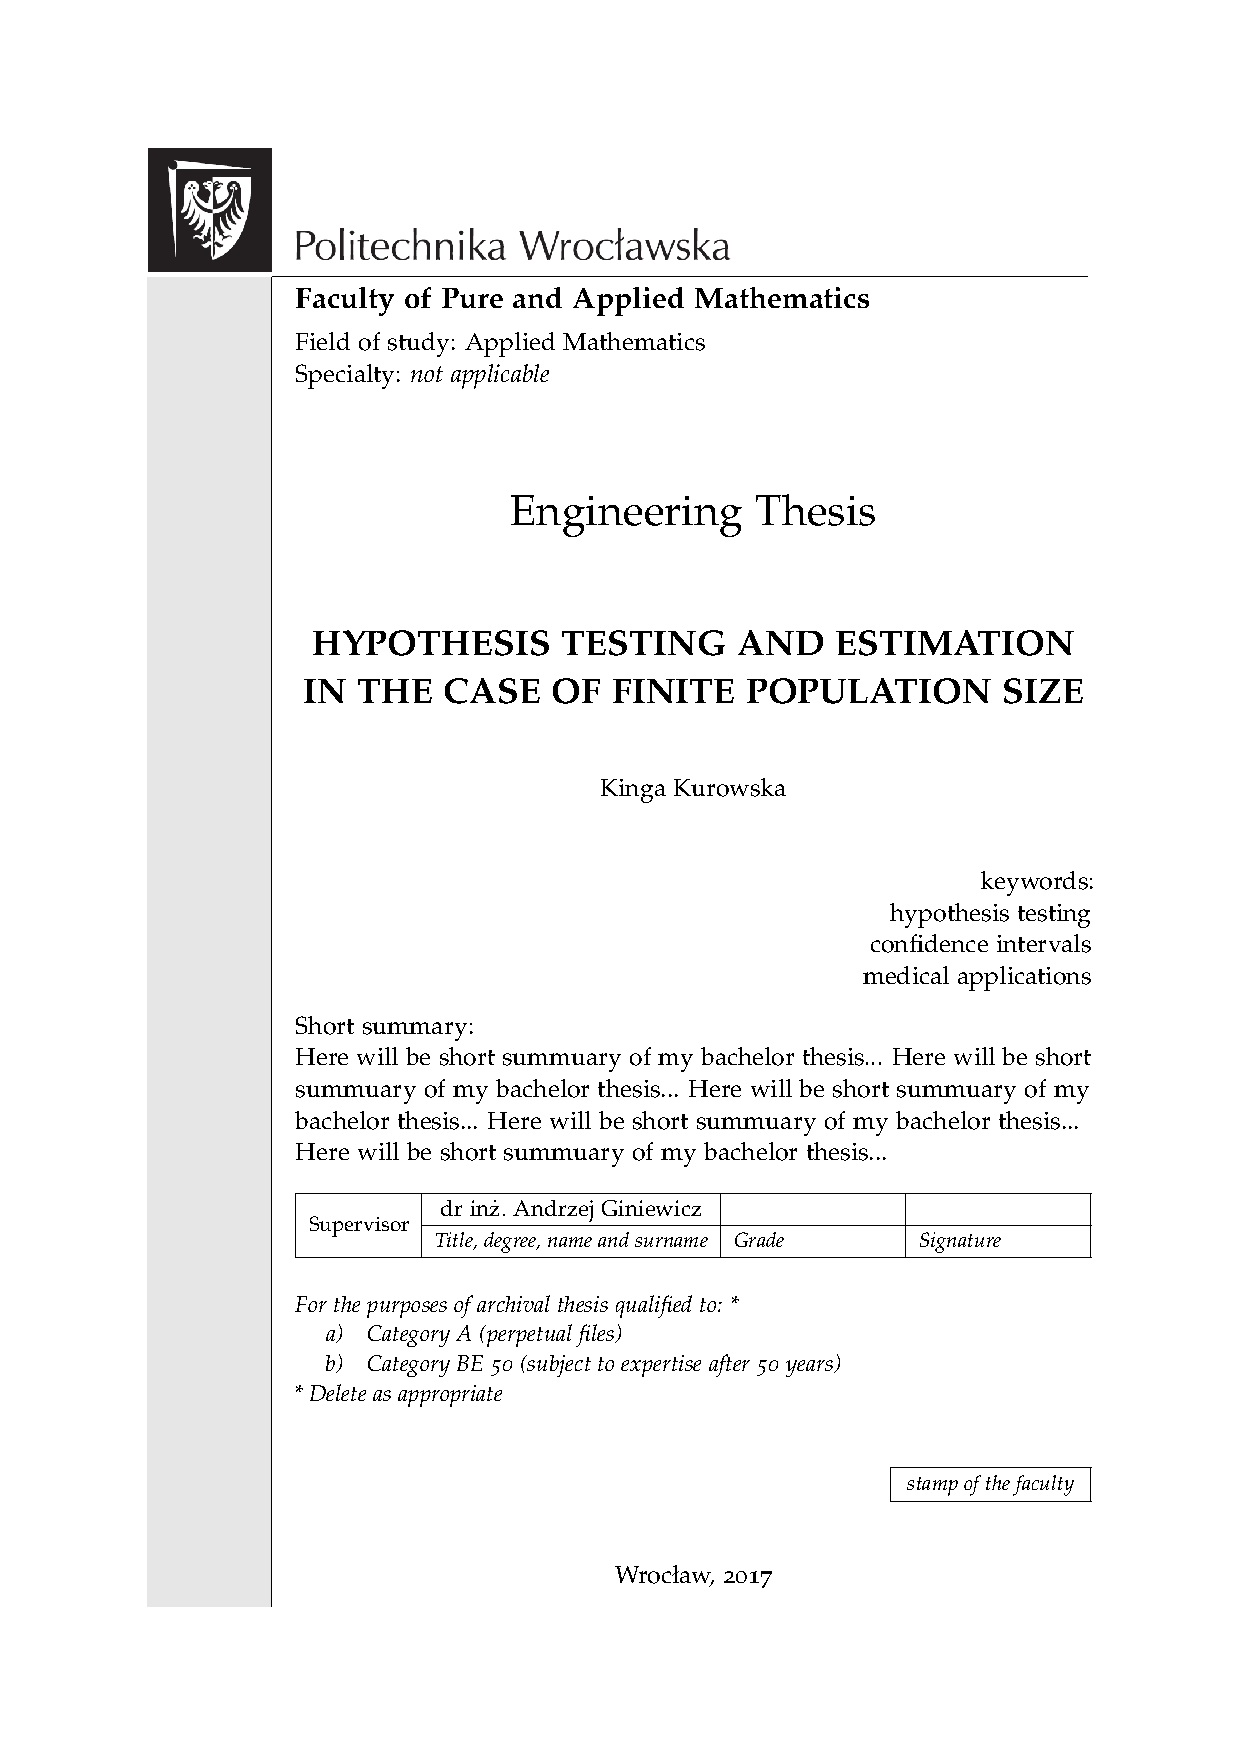
\includepdf{StronaTytulowa_ang.pdf}
\end{titlepage}


\tableofcontents

\chapter*{Wstęp}
Początki teorii rachunku prawdopodobieństwa i~statystyki sięgają XVI~w. Zajmowano się wtedy analizą rzutu kostką oraz prawdopodobieństwem błędów pomiarowych. Już w~XVII wieku Blaise Pascal sformułował i~dowiódł własności trójkąta arytmetycznego oraz użył pojęcia kombinacji~\cite{Hald2003}. Na początku XVIII~wieku opublikowane zostały prace Jacoba Bernoullego, w~których zawarł wiele swoich tez na temat prawdopodobieństwa. Przez te kilka wieków teoria rachunku prawdopodobieństwa i~statystyki znacząco się wzbogaciła i~rozwinęła. Rozpoczęto rozważania na temat estymacji i~testowania hipotez, które są w~naszych czasach zasadniczą domeną statystyki.

W przypadku dyskretnym najczęściej testowane są proporcje populacji~\cite{Lehmann1968}. Chcemy się przekonać czy dana próbka ma jakąś konkretną proporcję albo dwie próbki mają tę samą proporcję elementów z~badaną cechą. Znana jest powszechnie teoria dotycząca testowania hipotez, gdy populacja jest nieskończona, a~raczej na tyle duża, że możemy ją w przybliżeniu uznać za nieskończoną. Wtedy schemat próbkowania jest opisany jako losowanie ze zwracaniem. Jednak przypadek nieskończonej populacji nie wyczerpuje tematu testowania proporcji. Gdy populacja jest bardzo mała albo, gdy próbka jest niewiele mniejsza od całej populacji, schemat próbkowania opiera się o~losowanie bez zwracania. 

Warto zająć się teorią testowania hipotez dla skończonej populacji, ponieważ w~określonych przypadkach testy ze skończoną poprawką dają dużo dokładniejszą informację o~badanym przypadku niż testy zakładające nieskończoną populację. Ponadto zastosowanie tego typu testów ma duże znaczenie w~medycynie, gdzie często rozważane populacje mają na tyle wyspecjalizowane cechy, że są uważane za małe.

W~pierwszym rozdziale znajduje się opis schematu pobierania danych, w~przypadku nieskończonej i~skończonej populacji, oraz porównanie obu sposobów w~oparciu o~własności rozkładów próbek i~estymację przedziałową proporcji. W rozdziale~\ref{r2} przedstawiono testy bez skończonej poprawki oraz z~jej uwzględnieniem. Rozdział~\ref{r3} zawiera porównanie testów na podstawie prawdopodobieństwa błędu I~rodzaju oraz mocy testu. Na końcu pracy znajduje się podsumowanie uzyskanych wyników.
\chapter{Przedstawienie testów}

W tym rozdziale chciałabym opisać dwa testy wykorzystujące rozkład hipergeometryczny oraz test oparty na rozkładzie dwumianowym. Omówię także sposób liczenia prawdopodobieństwa błędu I rodzaju i mocy testu.

\section{Sformułowanie problemu}
Załóżmy, że $X_1$ i $X_2$ są niezależnymi zmiennymi losowymi o rozkładzie hipergeometrycznym $X_1\sim h(n_1,M_1,N_1)$, $X_2\sim h(n_2,M_2,N_2)$. Zaobserwowane wartości $X_1$ i $X_2$ oznaczmy odpowiednio $k_1$ i $k_2$ oraz proporcje $p_1=M_1/N_1$, $p_2=M_2/N_2$. Będę zajmować się testowaniem hipotez
\begin{equation}
H_0{:}\ p_1=p_2\quad \text{przeciwko} \quad H_1{:}\ p_1\neq p_2,
\end{equation}
w oparciu o $(k_1,n_1,N_1)$ i $(k_2,n_2,N_2)$.
Rozważmy unormowaną statystykę
\begin{equation}
Z_{X_1,X_2} = \frac{X_1/n_1-X_2/n_2}{\sqrt{V_{X_1,X_2}}},
\end{equation}
gdzie estymator wariancji pod warunkiem zachodzenia $H_0$ jest równy
\begin{equation}
V_{X_1,X_2} = \left(\frac{N_1-n_1}{n_1(N_1-1)}+\frac{N_2-n_2}{n_2(N_2-1)}\right)\left(\frac{X_1+X_2}{n_1+n_2}\right)\left(1-\frac{X_1+X_2}{n_1+n_2}\right).
\end{equation}
Wartość statystyki dla $k_1$ i $k_2$ będę oznaczać jako $Z_{k_1,k_2}$. Jest ona wyliczana według powyższych wzorów, zamieniając $X_1$ i $X_2$ wartościami obserwacji.

\section{Test Z}
Ten test jest oparty na centralnym twierdzeniu granicznym, które mówi, że pod warunkiem $H_0$ w przybliżeniu rozważana statystyka $Z_{X_1,X_2}$ jest z rozkładu normalnego standaryzowanego $N(0,1)$. Wtedy $p$-wartość wyraża się wzorem
\begin{equation}
P(|Z_{X_1,X_2}|\geq|Z_{k_1,k_2}|\ |H_0) = 2(1-\Phi(|Z_{k_1,k_2}|)),
\end{equation}
gdzie $\Phi()$ oznacza dystrybuantę rozkładu $N(0,1)$. Test Z odrzuca hipotezę zerową, gdy $p$-wartość jest mniejsza od poziomu istotności $\alpha$.

\section{Test E}
W tym przypadku opieramy się o rzeczywistą $p$-wartość, która jest równa
\begin{equation}
\label{realpvalue}
\begin{split}
P(|Z_{X_1,X_2}|\geq|Z_{k_1,k_2}|\ |H_0) =& E_{X_1,X_2}(\1{|Z_{X_1,X_2}|\geq|Z_{k_1,k_2}|}\ |H_0) = \\
= \sum_{x_1=L_1}^{U_1}\sum_{x_2=L_2}^{U_2}& h(x_1;n_1,N_1p,N_1)h(x_2;n_2,N_2p,N_2)\1{|Z_{X_1,X_2}|\geq|Z_{k_1,k_2}|},
\end{split}
\end{equation}
gdzie $E_{X_1,X_2}$ to wartość oczekiwana łącznego rozkładu $(X_1,X_2)$, a $p$ jest nieznaną wspólną proporcją pod warunkiem $H_0$. Nie jest możliwe policzenie $p$-wartości wprost ze wzoru (\ref{realpvalue}), ponieważ nie znamy parametru proporcji $p$. W artykule \cite{K.Krishnamoorthy2002} zaproponowany jest estymator $p$-wartości
\begin{equation}
\label{estpvalue}
\begin{split}
P(|Z_{X_1,X_2}|\geq|Z_{k_1,k_2}|\ |H_0) =& \\ =\sum_{x_1=L_{x_1}}^{U_{x_1}}\sum_{x_2=L_{x_2}}^{U_{x_2}}& h(x_1;n_1,\hat{M_1},N_1)h(x_2;n_2,\hat{M_2},N_2)\1{|Z_{X_1,X_2}|\geq|Z_{k_1,k_2}|},
\end{split}
\end{equation}
przy czym $\hat{p}=(k_1+k_2)/(n_1+n_2)$, $\hat{M_i}=[N_i\hat{p}]$, $L_{x_i}=\max\{0,\hat{M_i}-N_i+n_i\}$, $U_{x_i}=\min\{n_i,\hat{M_i}\}$, $i=1,2$. Test odrzuca $H_0$ wtedy, gdy $p$-wartość wyliczona wg wzoru (\ref{estpvalue}) jest mniejsza od poziomu istotności $\alpha$.

\section{Błąd I rodzaju}
Błąd I rodzaju to odrzucenie hipotezy zerowej, gdy jest ona prawdziwa. Prawdopodobieństwo tego błędu można wyliczyć, losując próbki z populacji, gdy $p_1=p_2$ i sprawdzając, ile razy zostaną odrzucone. Dla dużej ilości próbek prawdopodobieństwo błędu I rodzaju powinno być w okolicy poziomu istotności testu.

\section{Moc testu}
Przypomnę, że moc testu to prawdopodobieństwo odrzucenia hipotezy zerowej, gdy jest ona nieprawdziwa. Toteż jest ona wyznacznikiem dobrego testu. Większa wartość mocy oznacza lepszy test.

Moc obu testów można wyliczyć, korzystając z funkcji prawdopodobieństwa rozkładu hipergeometrycznego. Dla testu Z pod warunkiem hipotezy alternatywnej $H_1$ moc jest równa
\begin{equation}
\label{powerZ}
\sum_{k_1=L_1}^{U_1}\sum_{k_2=L_2}^{U_2} h(k_1;n_1,M_1,N_1)h(k_2;n_2,M_2,N_2)\1{|Z_{k_1,k_2}|>z_{1-\alpha/2}},
\end{equation}
gdzie $L_i=\max\{0,M_i-N_i+n_i\}$ i $U_i=\min\{n_i,M_i\}$, a $z_{1-\alpha/2}$ oznacza kwantyl rozkładu normalnego standardowego rzędu $1-\alpha/2$.

Tymczasem dla testu E moc zdefiniowana jest następująco
\begin{equation}
\begin{split}
&\sum_{k_1=L_1}^{U_1}\sum_{k_2=L_2}^{U_2} h(k_1;n_1,M_1,N_1)h(k_2;n_2,M_2,N_2) \times \\
& \times \1{\sum_{x_1=L_{x_1}}^{U_{x_1}}\sum_{x_2=L_{x_2}}^{U_{x_2}} h(x_1;n_1,\hat{M_1},N_1)h(x_2;n_2,\hat{M_2},N_2) \1{|Z_{X_1,X_2}|\geq|Z_{k_1,k_2}|}\leq\alpha },
\end{split}
\end{equation}
gdzie wszelkie parametry oznaczają to samo co we wzorach (\ref{estpvalue}) i (\ref{powerZ}).

\section{Test bez skończonej poprawki}
W tym przypadku zamiast rozkładu hipergeometrycznego używamy dwumianowego, a więc $X_1$ i $X_2$ są niezależnymi zmiennymi losowymi o rozkładzie Bernoullego $X_1\sim B(n_1,p_1)$, $X_2\sim B(n_2,p_2)$. Unormowana statystyka w tym przypadku przyjmuje postać
\begin{equation}
Z_{X_1,X_2} = \frac{X_1/n_1-X_2/n_2}{\sqrt{V_{X_1,X_2}}},
\end{equation}
gdzie estymator wariancji pod warunkiem $H_0$ jest równy
\begin{equation}
V_{X_1,X_2} = \sqrt{p(1-p)(1/n_1+1/n_2)},
\end{equation}
gdzie $p=(X_1+X_2)/(n_1+n_2)$.
Wartość statystyki $Z_{k_1,k_2}$ jest wyliczana według powyższych wzorów, wstawiając obserwacje $k_1$ i $k_2$ w miejsca zmiennych losowych.

Ten test jest, podobnie jak omówiony wcześniej test Z, oparty na centralnym twierdzeniu granicznym. Czyli rozważana statystyka $Z_{X_1,X_2}$ ma rozkład standardowy normalny $N(0,1)$. Wtedy $p$-wartość wyraża się wzorem
\begin{equation}
P(|Z_{X_1,X_2}|\geq|Z_{k_1,k_2}|\ |H_0) = 2(1-\Phi(|Z_{k_1,k_2}|)),
\end{equation}
Test odrzuca hipotezę zerową, gdy $p$-wartość jest mniejsza od poziomu istotności $\alpha$.

Prawdopodobieństwo błędu I rodzaju jest liczone analogicznie jak w przypadku poprzednich testów. Aczkolwiek moc testu jest liczona inaczej, ze względu na inny rozkład zmiennych losowych. W tym przypadku będzie ona równa
\begin{equation}
\sum_{k_1=0}^{n}\sum_{k_2=0}^{n} b(k_1;n_1,p_1)b(k_2;n_2,p_2)\1{|Z_{k_1,k_2}|>z_{1-\alpha/2}},
\end{equation}
przy czym $b(k;n,p)$ oznacza funkcję prawdopodobieństwa rozkładu dwumianowego określoną wzorem
\begin{equation}
b(k;n,p) = P(X=k) = \binom{n}{k} p^k (1-p)^{n-k},\ 0\leq k\leq n.
\end{equation}

\chapter{Przedstawienie testów}
\label{r2}
W niniejszym rozdziale znajduje się opis trzech testów. Dwa testy ze skończoną poprawką wykorzystują rozkład hipergeometryczny, a~trzeci, test bez skończonej poprawki, opiera się o~rozkład dwumianowy. Następnie omówiony jest sposób liczenia mocy dla wymienionych testów.

\section{Sformułowanie problemu}
Załóżmy, że $X_1$ i~$X_2$ są niezależnymi zmiennymi losowymi. Zaobserwowane wartości $X_1$ i~$X_2$ oznaczmy odpowiednio $k_1$ i~$k_2$ oraz proporcje w~obserwacjach $p_1$ i~$p_2$. Będziemy testować
\begin{equation}
H_0{:}\ p_1=p_2\quad \text{przeciwko} \quad H_1{:}\ p_1\neq p_2,
\end{equation}
na podstawie wartości obserwacji i~znanych parametrów populacji.
Rozważmy unormowaną statystykę
\begin{equation}
Z_{X_1,X_2} = \frac{X_1/n_1-X_2/n_2}{\sqrt{V_{X_1,X_2}}},
\end{equation}
gdzie $V_{X_1,X_2}$ to estymator wariancji rozkładu zmiennej losowej $X_1/n_1-X_2/n_2$, pod warunkiem prawdziwości $H_0$, w~połączonej próbie. Jego wzór zależy od rozkładu, z~którego pochodzą zmienne losowe $X_1$ i~$X_2$.
Wartość statystyki $Z_{X_1,X_2}$ oznaczmy jako $Z_{k_1,k_2}$. Jest ona wyliczana według powyższych wzorów, poprzez zamienienie zmiennych losowych $X_1$ i~$X_2$ odpowiednio ich wartościami $k_1$ i~$k_2$.

\section{Testy ze skończoną poprawką}
\label{r2:skonczonapoprawka}
Jak już było wspomniane w~podrozdziale \ref{r1:skonczonapopulacja}, próbki w~przypadku skończonej populacji pochodzą z~rozkładu hipergeometrycznego. Zatem $X_1\sim \mathcal{H}(n_1,M_1,N_1)$, $X_2\sim \mathcal{H}(n_2,M_2,N_2)$ oraz proporcje są równe $p_1=M_1/N_1$, $p_2=M_2/N_2$. Znane parametry to rozmiary próbek $n_1$ i~$n_2$ i~wielkości populacji $N_1$ i~$N_2$.

W celu wyprowadzenia wariancji rozkładu $X_1/n_1-X_2/n_2$ pod warunkiem $p_1=p_2$ w~połączonej próbie, zapiszmy wariancję rozważanej zmiennej losowej w~łącznej próbie, korzystając z~własności wariancji oraz tego, że $Cov(X_1,X_2)=0$ z~niezależności $X_1$ i~$X_2$
\begin{equation}
Var(X_1/n_1-X_2/n_2)=Var(X_1/n_1) + Var(X_2/n_2) = Var(X_1)/n_1^2+Var(X_2)/n_2^2.
\end{equation}
Wariancje $X_1$ i~$X_2$ są równe
\begin{align}
Var(X_1)=n_1 p_1 (1-p_1)(N_1-n_1)/(N_1-1),\\
Var(X_2)=n_2 p_2 (1-p_2)(N_2-n_2)/(N_2-1).
\end{align}
Pamiętając, że zakładamy równość $p_1=p_2$ zastąpmy oba parametry jednym równym $p$. Po podstawieniu otrzymujemy
\begin{equation}
\begin{split}
V_{X_1,X_2} =& \frac{1}{n_1}p(1-p)\frac{N_1-n_1}{N_1-1} + \frac{1}{n_2}p(1-p)\frac{N_2-n_2}{N_2-1}= \\
=&p(1-p)\left(\frac{N_1-n_1}{n_1(N_1-1)}+\frac{N_2-n_2}{n_2(N_2-1)}\right),
\end{split}
\end{equation}
przy czym $p$ to proporcja liczby osobników z~daną cechą do całości populacji w~rozkładzie łącznym. Wobec czego $p=(X_1+X_2)/(n_1+n_2)$. Ostatecznie otrzymujemy
\begin{equation}
V_{X_1,X_2} = \left(\frac{N_1-n_1}{n_1(N_1-1)}+\frac{N_2-n_2}{n_2(N_2-1)}\right)\left(\frac{X_1+X_2}{n_1+n_2}\right)\left(1-\frac{X_1+X_2}{n_1+n_2}\right).
\end{equation}

\subsection{Test Z}
Test~Z jest oparty na centralnym twierdzeniu granicznym, według którego, rozważana statystyka $Z_{X_1,X_2}$, pod warunkiem prawdziwości $H_0$, jest w~przybliżeniu z~rozkładu standardowego normalnego $\mathcal{N}(0,1)$. Wtedy $p$-wartość wyraża się wzorem
\begin{equation}
P(|Z_{X_1,X_2}|\geq|Z_{k_1,k_2}|\ |H_0) \approx 2(1-\Phi(|Z_{k_1,k_2}|)),
\end{equation}
gdzie $\Phi$ oznacza dystrybuantę rozkładu $N(0,1)$. Test Z~odrzuca hipotezę zerową, gdy $p$-wartość jest mniejsza od poziomu istotności $\alpha$.

\subsection{Test E}
Test E opiera się o~rzeczywistą $p$-wartość, która, według artykułu K. Krishnamoorthy i~J. Thomson z~2002 roku, jest równa \cite{K.Krishnamoorthy2002}
\begin{equation}
\label{realpvalue}
\begin{split}
P(|Z_{X_1,X_2}|&\geq|Z_{k_1,k_2}|\ |H_0) = E_{X_1,X_2}(\1{|Z_{X_1,X_2}|\geq|Z_{k_1,k_2}|}\ |H_0) = \\
&= \sum_{x_1=L_1}^{U_1}\sum_{x_2=L_2}^{U_2} h(x_1;n_1,N_1p,N_1)h(x_2;n_2,N_2p,N_2)\1{|Z_{X_1,X_2}|\geq|Z_{k_1,k_2}|},
\end{split}
\end{equation}
gdzie $E_{X_1,X_2}$ to wartość oczekiwana łącznego rozkładu $(X_1,X_2)$, a~$p$ jest nieznaną wspólną proporcją pod warunkiem $H_0$. Nie jest możliwe policzenie $p$-wartości wprost ze wzoru (\ref{realpvalue}), ponieważ nie znamy parametru proporcji $p$. Krishnamoorthy i~Thomson (2002) zaproponowali estymator $p$-wartości \cite{K.Krishnamoorthy2002}
\begin{equation}
\label{estpvalue}
\begin{split}
P(|Z_{X_1,X_2}|\geq|Z_{k_1,k_2}|\ |H_0) \approx& \\ =\sum_{x_1=L_{x_1}}^{U_{x_1}}\sum_{x_2=L_{x_2}}^{U_{x_2}} h(x_1;&n_1,\hat{M_1},N_1)h(x_2;n_2,\hat{M_2},N_2)\1{|Z_{X_1,X_2}|\geq|Z_{k_1,k_2}|},
\end{split}
\end{equation}
przy czym $\hat{p}=(k_1+k_2)/(n_1+n_2)$, $\hat{M_i}=[N_i\hat{p}]$ oraz  $L_{x_i}=\max\{0,\hat{M_i}-N_i+n_i\}$, $U_{x_i}=\min\{n_i,\hat{M_i}\}$, $i=1,2$. Test odrzuca $H_0$ wtedy, gdy $p$-wartość wyliczona według wzoru (\ref{estpvalue}) jest mniejsza od poziomu istotności $\alpha$.

\subsection{Moc testu}
Moc testu to prawdopodobieństwo odrzucenia hipotezy zerowej, gdy jest ona nieprawdziwa. Wobec tego, spośród testów na zadanym poziomie istotności, interesują nas te o~najwyższej mocy.

Moc obu testów można wyliczyć, korzystając z~funkcji prawdopodobieństwa rozkładu hipergeometrycznego. Dla testu~Z pod warunkiem hipotezy alternatywnej $H_1$ moc, zgodnie z~rozważaniami Krishnamoorthy i~Thomson (2002), jest równa \cite{K.Krishnamoorthy2002}
\begin{equation}
\label{powerZ}
\sum_{k_1=L_1}^{U_1}\sum_{k_2=L_2}^{U_2} h(k_1;n_1,M_1,N_1)h(k_2;n_2,M_2,N_2)\1{|Z_{k_1,k_2}|>z_{1-\alpha/2}},
\end{equation}
gdzie $L_i=\max\{0,M_i-N_i+n_i\}$ i~$U_i=\min\{n_i,M_i\}$, a~$z_{1-\alpha/2}$ oznacza kwantyl rozkładu normalnego standardowego rzędu $1-\alpha/2$.

Natomiast dla testu E, według Krishnamoorthy i~Thomson (2002), moc zdefiniowana jest następująco \cite{K.Krishnamoorthy2002}
\begin{equation}
\begin{split}
&\sum_{k_1=L_1}^{U_1}\sum_{k_2=L_2}^{U_2} h(k_1;n_1,M_1,N_1)h(k_2;n_2,M_2,N_2) \times \\
&\times \1{\sum_{x_1=L_{x_1}}^{U_{x_1}}\sum_{x_2=L_{x_2}}^{U_{x_2}} h(x_1;n_1,\hat{M_1},N_1)h(x_2;n_2,\hat{M_2},N_2) \1{|Z_{x_1,x_2}|\geq|Z_{k_1,k_2}|}\leq\alpha },
\end{split}
\end{equation}
gdzie parametry są takie same jak we wzorach (\ref{estpvalue}) i~(\ref{powerZ}).

\section{Test bez skończonej poprawki}
Dla testu bez poprawki na skończony rozmiar populacji, zamiast rozkładu hipergeometrycznego stosujemy dwumianowy, więc $X_1$ i~$X_2$ są niezależnymi zmiennymi losowymi o~rozkładzie Bernoulliego $X_1\sim \mathcal{B}(n_1,p_1)$, $X_2\sim \mathcal{B}(n_2,p_2)$. Znane parametry to rozmiary próbek $n_1$ i~$n_2$.

Wariancję rozkładu $X_1/n_1-X_2/n_2$, pod warunkiem $p_1=p_2$, w~łącznej próbie możemy wyprowadzić analogicznie jak w~podrozdziale \ref{r2:skonczonapoprawka}, wychodząc od wariancji rozważanej zmiennej losowej
\begin{equation}
Var(X_1/n_1-X_2/n_2) = Var(X_1)/n_1^2+Var(X_2)/n_2^2.
\end{equation}
Wariancje $X_1$ i~$X_2$ są równe
\begin{align}
Var(X_1)=n_1 p_1 (1-p_1),\\
Var(X_2)=n_2 p_2 (1-p_2).
\end{align}
Zastępując $p_1$ i~$p_2$ jednym parametrem równym $p$, otrzymujemy
\begin{equation}
V_{X_1,X_2} = p(1-p)/n_1 + p(1-p)/n_2 = p(1-p)(1/n_1+1/n_2)
\end{equation}
przy czym $p=(X_1+X_2)/(n_1+n_2)$.

\subsection{Test Zb}

Test~Zb jest, podobnie jak omówiony wcześniej test E, oparty o~estymator $p$-wartości, który, zgodnie z~artykułem Storer i~Kim z~1990 roku, jest równy \cite{Storer1990}
\begin{equation}
P(|Z_{X_1,X_2}|\geq|Z_{k_1,k_2}|\ |H_0) \approx \sum_{x_1=0}^{n_1}\sum_{x_2=0}^{n_2} b(x_1;n_1,\hat{p_1})b(x_2;n_2,\hat{p_2})\1{|Z_{X_1,X_2}|\geq|Z_{k_1,k_2}|},
\end{equation}
gdzie $\hat{p}=(k_1+k_2)/(n_1+n_2)$.
Test odrzuca hipotezę zerową, gdy $p$-wartość jest mniejsza od poziomu istotności $\alpha$.

Moc testu wyraża się wzorem
\begin{equation}
\begin{split}
\sum_{k_1=0}^{n}\sum_{k_2=0}^{n} b(k_1;n_1,&p_1)b(k_2;n_2,p_2) \times \\
\times &\1{\sum_{x_1=0}^{n_1} \sum_{x_2=0}^{n_2} b(x_1;n_1,\hat{p_1}) b(x_2;n_2,\hat{p_2}) \1{|Z_{x_1,x_2}|\geq|Z_{k_1,k_2}|} \leq\alpha}.
\end{split}
\end{equation}


\chapter{Analiza testów}
\label{r3}

W celu porównania testów opisanych w~rozdziale \ref{r2}, napisano programy, które wyliczają prawdopodobieństwo błędu I~rodzaju i~moc testu oraz generują wykresy dla różnych parametrów.

\section{Porównanie testów ze skończoną poprawką}
\label{r3:skonczonetesty}
Na początku zostały porównane testy ze skończoną poprawką. Rysunek \ref{sizeZE_n} na stronie \pageref{sizeZE_n} przedstawia funkcję prawdopodobieństwa błędu I~rodzaju w~zależności od rozmiaru próbki dla różnych proporcji $p$. Po lewej stronie obserwacje z~obu populacji są tej samej wielkości $n_1=n_2=n$, natomiast po prawej różnią się, rozmiar pierwszej próbki ma ustaloną wartość. Pierwszym spostrzeżeniem jest to, że funkcja dla testu~E w~większości przypadków jest mniejsza niż dla testu Z. Dodatkowo dla testu~E prawdopodobieństwo błędu przekracza poziom istotności jedynie kilka razy i~to bardzo nieznacznie. Tymczasem dla testu~Z funkcja częściej przyjmuje wartości powyżej $\alpha$, dochodząc nawet do $0.95$, jak na wykresie \ref{sizeZE_p_0_05}. Warto wspomnieć także, że dla większych $p$ (0.1, 0.3) oraz wraz ze wzrostem wielkości próbki funkcje są bliżej siebie i~bardziej skupiają się przy poziomie istotności $\alpha$.

\begin{figure}[!h]
	\begin{subdiagrams}{sizeZE_p_0_05}{sizeZE_p_0_05_n1_5}
	\end{subdiagrams}
	
	\begin{subdiagrams}{sizeZE_p_0_1}{sizeZE_p_0_1_n1_10}
	\end{subdiagrams}
	
	\begin{subdiagrams}{sizeZE_p_0_3}{sizeZE_p_0_3_n1_5}
	\end{subdiagrams}
	\caption{Prawdopodobieństwo błędu I~rodzaju testów~Z i~E jako funkcja rozmiaru próbki $n$, przy zadanym poziomie istotności $\alpha=0.05$; $N_1=N_2=100$}
	\label{sizeZE_n}
\end{figure}

Rysunek \ref{sizeZE_p} na stronie \pageref{sizeZE_p} obrazuje również prawdopodobieństwo błędu I~rodzaju, ale w~zależności od proporcji $p$. Analizując wykresy funkcji, można dojść do analogicznych wniosków, jak dla rysunku \ref{sizeZE_n}. W~każdym przypadku prawdopodobieństwo błędu I~rodzaju testu~Z jest większe od prawdopodobieństwa błędu testu E. Oprócz tego funkcja dla testu~E przekracza poziom istotności jedynie na wykresie \ref{sizeZE_n1_30_n2_15}, podczas gdy funkcja błędu testu~Z tylko w~jednym przypadku (\ref{sizeZE_n1_10_n2_6}) pozostaje całkowicie poniżej $\alpha$.

Podsumowując, dla małych rozmiarów próbek test~Z nie jest na poziomie istotności $\alpha$, co wynika z~zastosowania centralnego twierdzenia granicznego w~wyliczaniu $p$-wartości. Przybliżenie rozkładem normalnym działa dobrze tylko dla dużych prób. Wobec czego test~Z zbyt często odrzuca hipotezę zerową, gdy jest ona prawdziwa. 

Rysunek \ref{powerZE_n} na stronie \pageref{powerZE_n} zawiera wykresy mocy obu testów w~zależności od rozmiaru próbki dla różnych proporcji oraz rozmiarów populacji. Druga populacja ma ustaloną proporcję $p_2$, a~pierwsza przyjmuje trzy wartości różne od $p_2$. Dla obu testów zauważalny jest wzrost mocy wraz ze zwiększaniem się rozmiaru próbki. Ponadto moc testu wzrasta także dla proporcji bardziej oddalonych od siebie. W~każdym przypadku, dla próby $n=50$ i~różnicy między proporcjami $0.3$, moce mają wartość bliską $1$. 

Porównując, moc testu~Z jest większa od mocy testu E, jednakże różnice nie są znaczne. Ponadto, z~analizy błędu I~rodzaju, wiemy, że test~Z zbyt często odrzuca $H_0$, co wpływa na wyższą moc testu. Natomiast test~E utrzymuje poziom istotności $\alpha$, wobec czego niewiele mniejsza moc testu nie oznacza, że test~E jest gorszy. Wprost przeciwnie, patrząc na wartości prawdopodobieństwa błędu I~rodzaju, test~E jest poprawny, podczas gdy test~Z nie spełnia swojej roli.

\begin{figure}[H]
	\begin{subdiagrams}{sizeZE_n_10}{sizeZE_n1_10_n2_6}
	\end{subdiagrams}
	
	\begin{subdiagrams}{sizeZE_n_20}{sizeZE_n1_20_n2_5}
	\end{subdiagrams}
	
	\begin{subdiagrams}{sizeZE_n_30}{sizeZE_n1_30_n2_15}
	\end{subdiagrams}
	\caption{Prawdopodobieństwo błędu I~rodzaju testów~Z i~E jako funkcja proporcji $p=M_1/N_1=M_2/N_2$, przy zadanym poziomie istotności $\alpha=0.05$; $N_1=N_2=100$}
	\label{sizeZE_p}
\end{figure}


\begin{figure}[H]
	\begin{subdiagram}{powerZE_N1_30_N2_50_p_0_6}
	\end{subdiagram}
	\begin{subdiagram}{powerZE_N_100_p_0_1}
	\end{subdiagram}
	\begin{subdiagram}{powerZE_N1_100_N2_200_p_0_1}
	\end{subdiagram}
	\begin{subdiagram}{powerZE_N1_3000_N2_100_p_0_6}
	\end{subdiagram}
	
	\caption{Moc testów~Z i~E jako funkcja rozmiaru próbki $n$}
	\label{powerZE_n}
\end{figure}

\newpage

\section{Porównanie testu bez skończonej poprawki~Zb z~testem E}

W niniejszym podrozdziale porównano test~Zb z~testem E. Nie włączono do analizy testu Z, z~powodu wniosków opisanych w~podrozdziale \ref{r3:skonczonetesty}. Poniższe rozważania zostały przeprowadzone, aby potwierdzić zasadność stosowania testu ze skończoną poprawką dla małych populacji lub o~stosunkowo dużej próbie.

Na rysunku \ref{sizeZbE_n} umieszczonym ne stronie \pageref{sizeZbE_n} znajdują się wykresy prawdopodobieństwa błędu I~rodzaju analizowanych testów. Test E, jak stwierdzono w~podrozdziale \ref{r3:skonczonetesty}, nie przekracza poziomu istotności $\alpha$. Jednakże dla testu~Zb prawdopodobieństwo błędu I~rodzaju znacząco przekracza poziom istotności. Funkcja błędu~Zb przyjmuje wartości bliskie $0.2$, gdzie największa znajduje się na wykresie \ref{sizeZbE_p_0_1_n1_10}. Warto wspomnieć także, że funkcja jest największa w~przypadku małych próbek. Na wykresach \ref{sizeZbE_p_0_3} i~\ref{sizeZbE_p_0_3_n1_5} widać, że mniej więcej do $n=20$ test~Zb jest powyżej poziomu $\alpha$, następnie oscyluje, podobnie jak test E, w~okolicach poziomu istotności. 

Podsumowując, test~Zb nie jest adekwatny do rozważanego przypadku gdy wartość $n$ jest mała. Odrzuca hipotezę zerową dużo częściej, niż powinien test na poziomie $\alpha$. Jest to spowodowane użyciem rozkładu dwumianowego w~formułowaniu statystyki testowej. Faktycznie dla dużych próbek różnica jest nieznaczna, natomiast w~sytuacji małej próbki rozbieżności są bardzo widoczne.

\begin{figure}[!h]
	\begin{subdiagrams}{sizeZbE_p_0_05}{sizeZbE_p_0_05_n1_5}
	\end{subdiagrams}
	
	\begin{subdiagrams}{sizeZbE_p_0_1}{sizeZbE_p_0_1_n1_10}
	\end{subdiagrams}
	
	\begin{subdiagrams}{sizeZbE_p_0_3}{sizeZbE_p_0_3_n1_5}
	\end{subdiagrams}
	\caption{Prawdopodobieństwo błędu I~rodzaju testów~Zb i~E jako funkcja rozmiaru próbki $n$, przy zadanym poziomie istotności $\alpha=0.05$; $N_1=N_2=100$}
	\label{sizeZbE_n}
\end{figure}

Rysunek \ref{powerZbE_n} na stronie \pageref{powerZbE_n} przedstawia wykresy mocy rozważanych testów w~zależności od rozmiaru próbki dla różnych rozmiarów populacji oraz proporcji $p$. Moc testu~Zb jest niewiele większa od mocy testu E. Jednakże, podobnie jak w~przypadku testu Z, wynika to ze zbyt częstego odrzucania~$H_0$. Biorąc pod uwagę ten fakt wyższa wartość testu~Zb nie świadczy o~jego poprawności.

\begin{figure}[!h]
	\begin{subdiagram}{powerZbE_N1_30_N2_50_p_0_6}
	\end{subdiagram}
	\begin{subdiagram}{powerZbE_N_100_p_0_1}
	\end{subdiagram}
	\begin{subdiagram}{powerZbE_N1_100_N2_200_p_0_1}
	\end{subdiagram}
	\begin{subdiagram}{powerZbE_N1_3000_N2_100_p_0_6}
	\end{subdiagram}

	\caption{Moc testów~Zb i~E jako funkcja rozmiaru próbki $n$}
	\label{powerZbE_n}
\end{figure}

Ostatecznie pokazano, że test bez skończonej poprawki nie powinien być stosowany w~przypadku małej populacji, ponieważ wtedy znacznie przekracza poziom istotności $\alpha$. Najlepszym testem dla skończonej populacji okazał się test E, który dla różnych przypadków utrzymuje poziom istotności $\alpha$. 

\listoffigures
%\listoftables

\bibliographystyle{unsrt}
%\bibliographystyle{abbrv}
\bibliography{dokument_KK}
	
\end{document}